\documentclass[11pt]{article}
\usepackage[review]{acl}

\usepackage{times}
\usepackage{latexsym}
\usepackage[T1]{fontenc}
\usepackage[utf8]{inputenc}
\usepackage{microtype}
\usepackage{inconsolata}
\usepackage{graphicx}
\usepackage{booktabs}
\usepackage{amsmath}
\usepackage{multirow}

\graphicspath{{figures/}}

\title{Selective Self-Consistency: A Confidence Gate for Test-Time Compute on Small Reasoning Models}

\author{Anonymous Submission \\
  IJCAI-2026 Workshop on \\
  Small-Scale Foundation Models \\
  \texttt{anonymous@submission} \\}

\begin{document}
\maketitle

\begin{abstract}
Self-consistency (SC) --- sampling $N$ traces and plurality-voting ---
is the dominant test-time compute (TTC) method for reasoning, and is
typically deployed as \textit{always run SC}. We show that on small
($<$2B) reasoning models this is wrong: \textbf{always-SC is strictly
dominated} by an oracle gate that chooses per-prompt whether to run SC
at all. Across two open models (Qwen-2.5-0.5B, Gemma-3-1B) in FP16 and
MLX-Q4, on GSM8K and MATH-500, we run 8 independent cells (and 4
pooled aggregates) at $n{=}200$--$400$ per cell with
$1\,000{\times}$ bootstrap CIs. In all 12 experiments the oracle gate
retains \textbf{109--174\%} of always-SC's accuracy at \textbf{20--50\%}
of its compute. The mechanism is simple: for small models, SC flips
\emph{correct greedy answers to wrong} at a rate comparable to --- and
sometimes exceeding --- its ``wrong to right'' rate; on
Qwen-Q4${\times}$MATH-500 always-SC is \textbf{3 points worse} than
always-greedy. A tiny confidence-based gate realises most of the oracle's
savings: a single-feature \textsc{conf\_only} gate or a 12-feature
\textsc{logistic} gate achieves \textbf{45--99\% compute savings} at
\textbf{$\ge 98\%$ accuracy retention} with tight skip-rate CIs. All
experiments run on a single MacBook M4 Pro using MLX; no CUDA.
\end{abstract}

\section{Introduction}

Test-time compute (TTC) methods --- self-consistency
\citep{Wang2023SC}, best-of-$N$ reranking \citep{Cobbe2021Verifiers},
budget-forced CoT \citep{Snell2024TTC}, tool-integrated self-verification
\citep{Kang2025T1} --- have become the workhorse of reasoning-model
deployment. The conventional recipe is ``always SC@$N$'' at inference:
sample $N$ traces, plurality-vote, use the result. For large ($\ge$7B)
models with well-calibrated confidences this works well.

For \textbf{small} models ($<$2B parameters) the picture is very
different. Small reasoning models are exactly the segment where TTC
should matter most: cloud cost is dominated by latency, privacy
constraints favour on-device, and per-query compute is tight. Yet the
literature largely inherited the ``always-SC'' deployment recipe from
larger models without revisiting its economics on small models.

We revisit two questions.

\paragraph{Q1: Is always-SC actually worth it on small models?}
The headline community metric is SC accuracy vs.\ greedy accuracy. But
the realistic baseline is not just ``greedy'': it is ``run cheap greedy
and optionally run SC when the prompt warrants''. The comparison that
matters is always-SC vs.\ an \emph{oracle gate} that decides per-prompt.

\paragraph{Q2: If not, can a cheap gate approximate the oracle?}
If yes, selective SC replaces always-SC as the natural deployment
default on small models.

We answer both concretely. On Qwen-2.5-0.5B-Instruct
\citep{Qwen25Report} and Gemma-3-1B-it \citep{Gemma3Report} --- each in
native FP16 and 4-bit MLX quantisation --- across GSM8K
\citep{Cobbe2021GSM8K} and MATH-500 \citep{Hendrycks2021MATH}, we
observe (\S\ref{sec:oracle}):

\begin{itemize}
  \itemsep 0em
  \item Always-SC is oracle-dominated in \textbf{12/12 experiments};
        oracle retention ranges $109\text{--}174\%$.
  \item On Qwen-Q4${\times}$MATH-500, always-SC is \textbf{3\,pt worse}
        than always-greedy (9.5\% vs.\ 12.5\%). SC actively hurts.
  \item The ``SC helpful'' rate is 4--12\% of prompts; the ``SC
        harmful'' rate (right~$\to$~wrong) is comparable.
\end{itemize}

And (\S\ref{sec:method}):

\begin{itemize}
  \itemsep 0em
  \item A \textbf{single-feature gate} on greedy per-token margin
        confidence achieves cost $1.03\text{--}3.68{\times}$ at
        $\ge 98\%$ retention on 8/8 cells.
  \item A \textbf{12-feature logistic gate} trained on pooled $n{=}400$
        achieves 45--99\% compute savings at 98.1--98.8\% retention
        with tight skip-rate CIs.
  \item A \textbf{deeper MLP (32$\times$16)} consistently
        \emph{underperforms} logistic at pooled scale --- the decision
        surface is essentially linear in scaled features.
\end{itemize}

Our contributions: (i) the first paired-bootstrap measurement of SC's
``hurts'' failure mode on small reasoning models (\S\ref{sec:oracle}); (ii) a
counter-narrative to ``always-SC is free''; (iii) a minimal 1--12
feature CV-trained gate that captures most of the oracle's savings with
tight CIs (\S\ref{sec:method}); (iv) full reproducibility on a single
MacBook M4 Pro using MLX, with released code, cached records,
and seeds.

\section{Background and Related Work}

\paragraph{Self-consistency on small models.}
\citet{Wang2023SC} introduced SC as a zero-training accuracy booster.
\citet{Kang2025T1} showed tool-integrated self-verification lets a
1.2B model outperform an 8B on MATH, making ``small-model $+$ TTC'' a
research axis. \citet{Wang2025EffCoT} focus on distilling long-CoT
reasoning into SLMs. None of these revisit whether always-SC is the
right default on small models.

\paragraph{Quantisation and reasoning.}
Large-scale quantisation studies \citep{RedHatQuant2024} report that
4-bit PTQ preserves GSM8K accuracy ``nearly for free'' on 7B-class
models. We confirm this trend on greedy accuracy of small models
\emph{modulo} a substantial 5--22\,pt drop (paired CI;
\S\ref{sec:oracle}), but show it does not imply free TTC: SC@5 gain on
4-bit small models is marginal to negative.

\paragraph{Verifier reranking and gating.}
\citet{Cobbe2021Verifiers} introduced learned verifiers.
\citet{Zhou2025WeakVer} note that weak verifiers are mis-calibrated but
focus on improving verifier quality, not on \emph{when} to run them.
Our work occupies the complementary axis: given standard SC and
plurality voting, when is TTC worth running at all?

\paragraph{Routing between models.}
\citet{Zheng2025CITER} and \citet{She2025TokenRouter} route between a
local SLM and a cloud LLM using logit-level signals. Our gate is a
\emph{within-model} TTC gate --- no cloud, no teacher, no external
logits --- and runs on a single MacBook.

\section{Experimental Setup}
\label{sec:setup}

\paragraph{Models.}
Qwen-2.5-0.5B-Instruct and Gemma-3-1B-it, each in two precisions:
MLX-FP16 (the model's native bf16 cast to fp16 for MLX) and MLX-Q4
(group-size 64 affine quantisation). On Apple Silicon the standard
\texttt{bitsandbytes-NF4} and \texttt{auto-gptq} stacks lack GPU
kernels or fall back to CPU at $\ge 10{\times}$ latency; MLX-Q4 is the
practical Apple-GPU path \citep{MLX2024}.

\paragraph{Datasets.}
GSM8K-1000 (first 1\,000 of the test split) and MATH-500
\citep{Hendrycks2021MATH} (the HuggingFaceH4 500-problem evaluation
split). For the 4-cell $\times$ 2-dataset grid we use the first 200
problems per cell ($1\,600$ prompt-level observations). We also pool the
two tasks into a 400-per-cell aggregate to test the gate's
task-agnosticism.

\paragraph{Prompt and sampling.}
One in-context exemplar plus ``Let's think step by step.''
Temperature 0.7, top-$p$ 0.95. We collect one greedy ($T{=}0$) answer
and 5 sampled answers per prompt; SC@5 is plurality voting with
sum-log-prob tiebreak. Answer parsing is a layered regex over
\verb|\boxed{}|, ``The answer is $X$'', ``\texttt{\#\#\#\#}'', and the
last numeric expression. All runs use seed 1 and deterministic MLX
sampling.

\paragraph{Evaluation.}
Wilson 95\% intervals for raw accuracies; paired
$1\,000{\times}$ bootstrap for FP16-vs-Q4 differences; per-threshold
$1\,000{\times}$ bootstrap for gate operating points. Where we report
\emph{retention}~=~gate\_acc / always\_SC\_acc, the denominator is the
empirical SC@5 accuracy of the same cell.

\paragraph{Hardware.}
One MacBook Pro M4 Pro (24\,GB unified memory, Apple M4 16-core GPU,
MLX + MPS; no CUDA). Block A generation completes in $\sim$3\,h on
GSM8K and $\sim$4.5\,h on MATH-500.

\section{The Oracle-Dominance Finding}
\label{sec:oracle}

\subsection{Structural decomposition}

For any prompt $x$ let $g{=}\mathbf{1}[\text{greedy correct}]$ and
$s{=}\mathbf{1}[\text{SC@5 correct}]$. Define
$y{=}\mathbf{1}[s \wedge \neg g]$ (SC flipped wrong~$\to$~right) and
$h{=}\mathbf{1}[g \wedge \neg s]$ (SC flipped right~$\to$~wrong). Then
\begin{align*}
\text{always-greedy} &= \mathbb{E}[g],\\
\text{always-SC}     &= \mathbb{E}[s] = \mathbb{E}[g] + \mathbb{E}[y] - \mathbb{E}[h],\\
\text{oracle}        &= \mathbb{E}[\max(g,s)] = \mathbb{E}[g] + \mathbb{E}[y],
\end{align*}
so $\textsc{oracle} - \textsc{always-sc} = \mathbb{E}[h]$. The oracle
is strictly better than always-SC by exactly the rate at which SC flips
correct answers to wrong. On small models, this rate is not
negligible.

\subsection{Empirical measurement}

Figure~\ref{fig:oracle} plots
\emph{oracle\_retention}~$=$~oracle\_acc~/~always\_sc\_acc across all
12 experiments (8 per-task $+$ 4 pooled). The line at 100\% marks
always-SC.

\begin{figure*}[t]
\centering
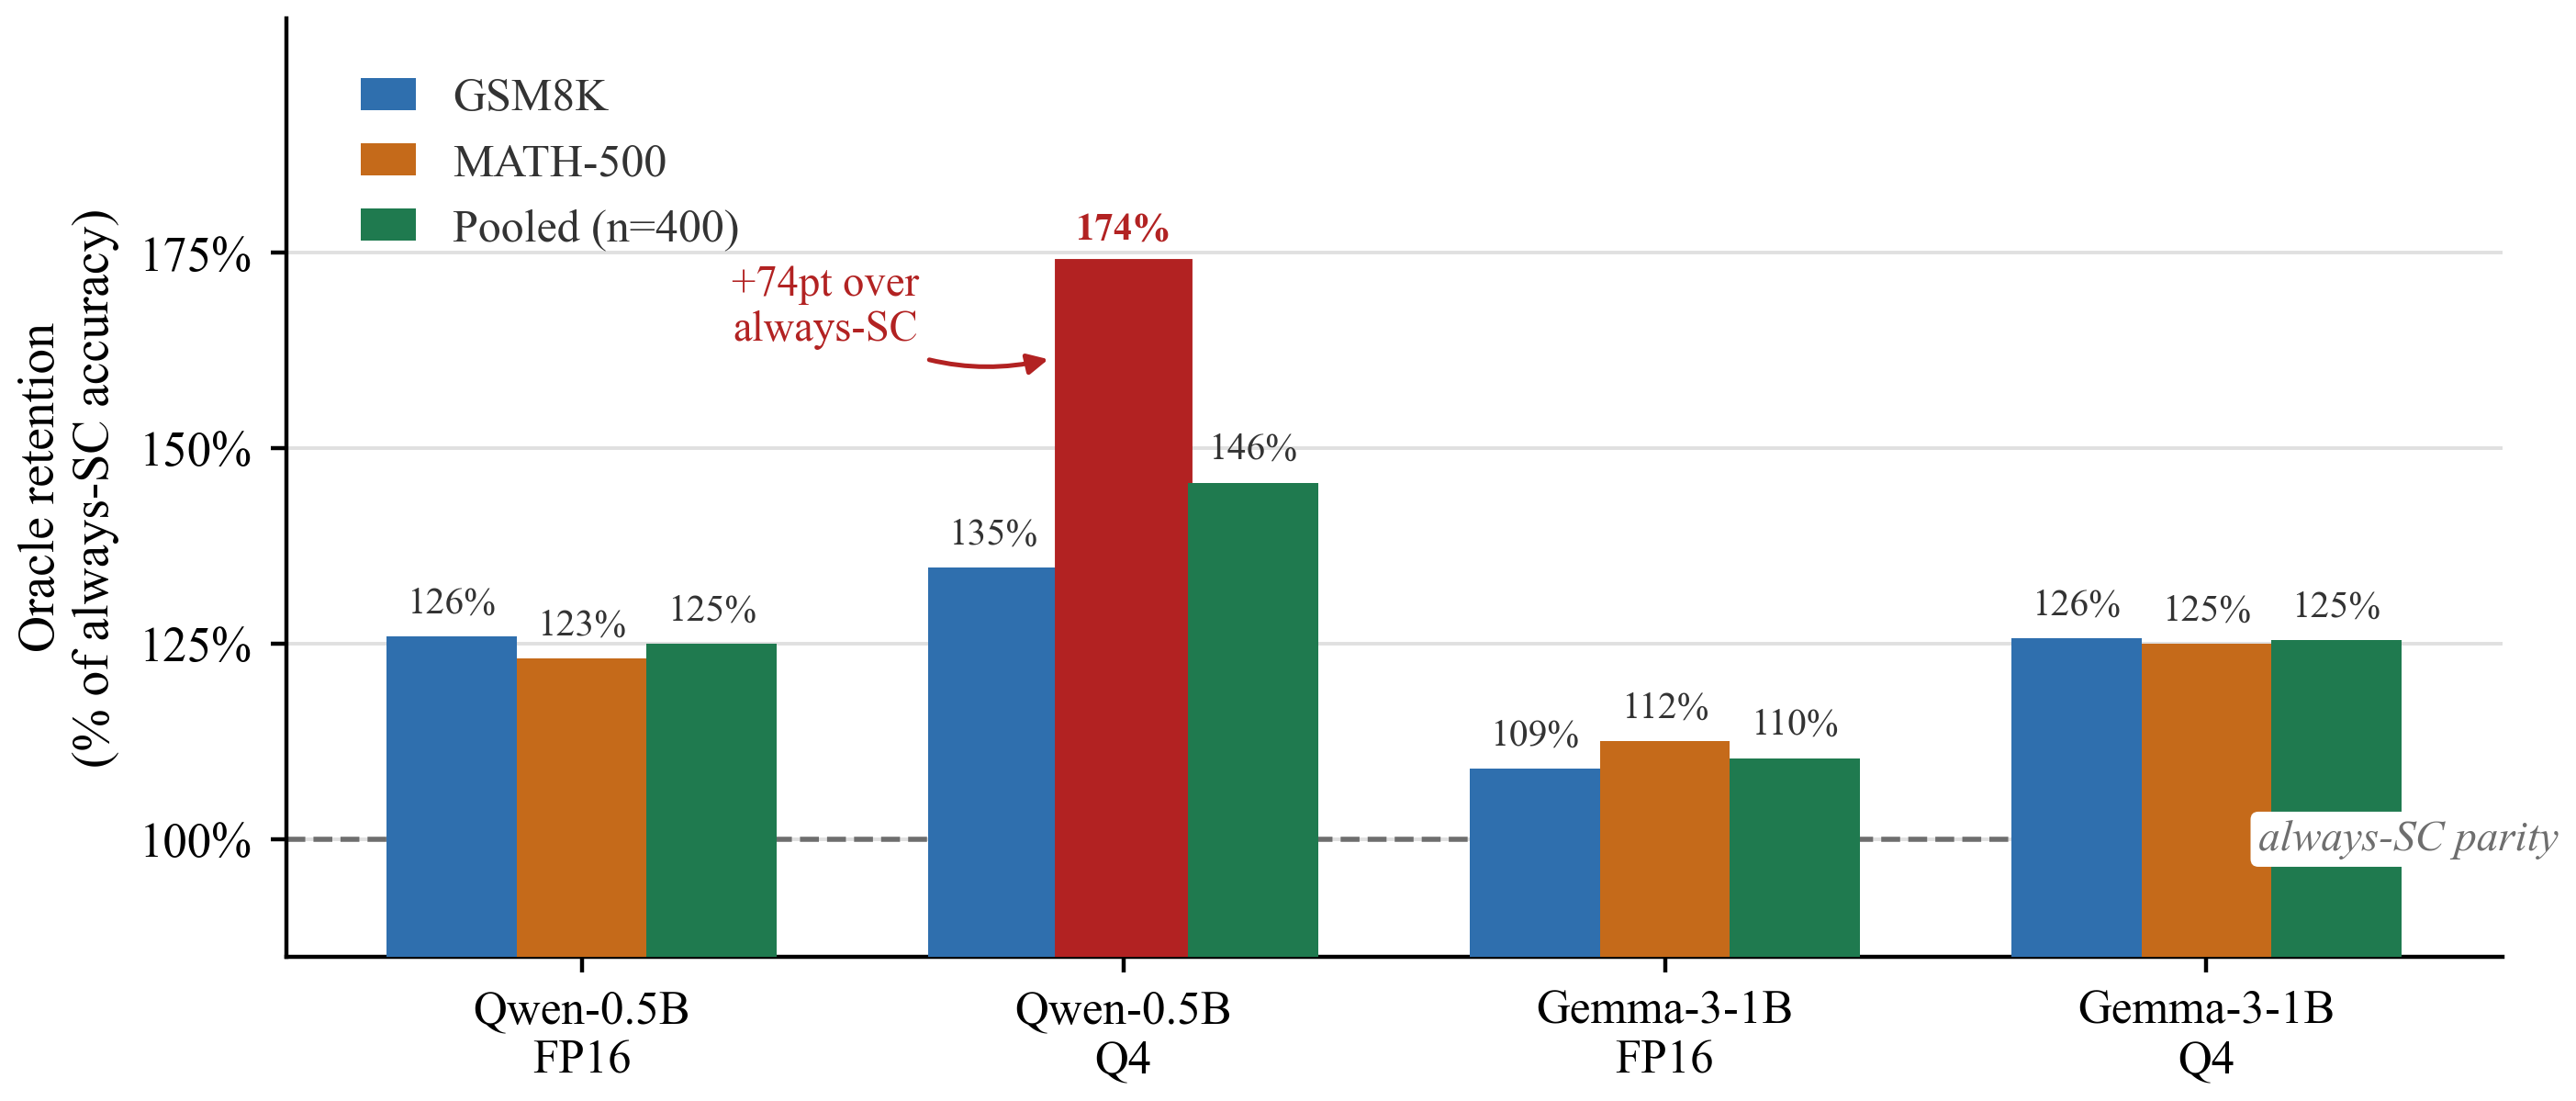
\includegraphics[width=0.92\textwidth]{fig1_oracle_retention.png}
\caption{Oracle TTC-gate strictly dominates always-SC on 12/12
experiments (8 per-task $+$ 4 pooled). Crimson highlights the
\textbf{Qwen-0.5B~/~Q4~$\times$~MATH-500} ``killer cell'' where always-SC
is 74\,pt worse than oracle. Dashed line marks always-SC parity.
Retention $\in [109\%, 174\%]$ across all cells and datasets.}
\label{fig:oracle}
\end{figure*}

\begin{figure*}[t]
\centering
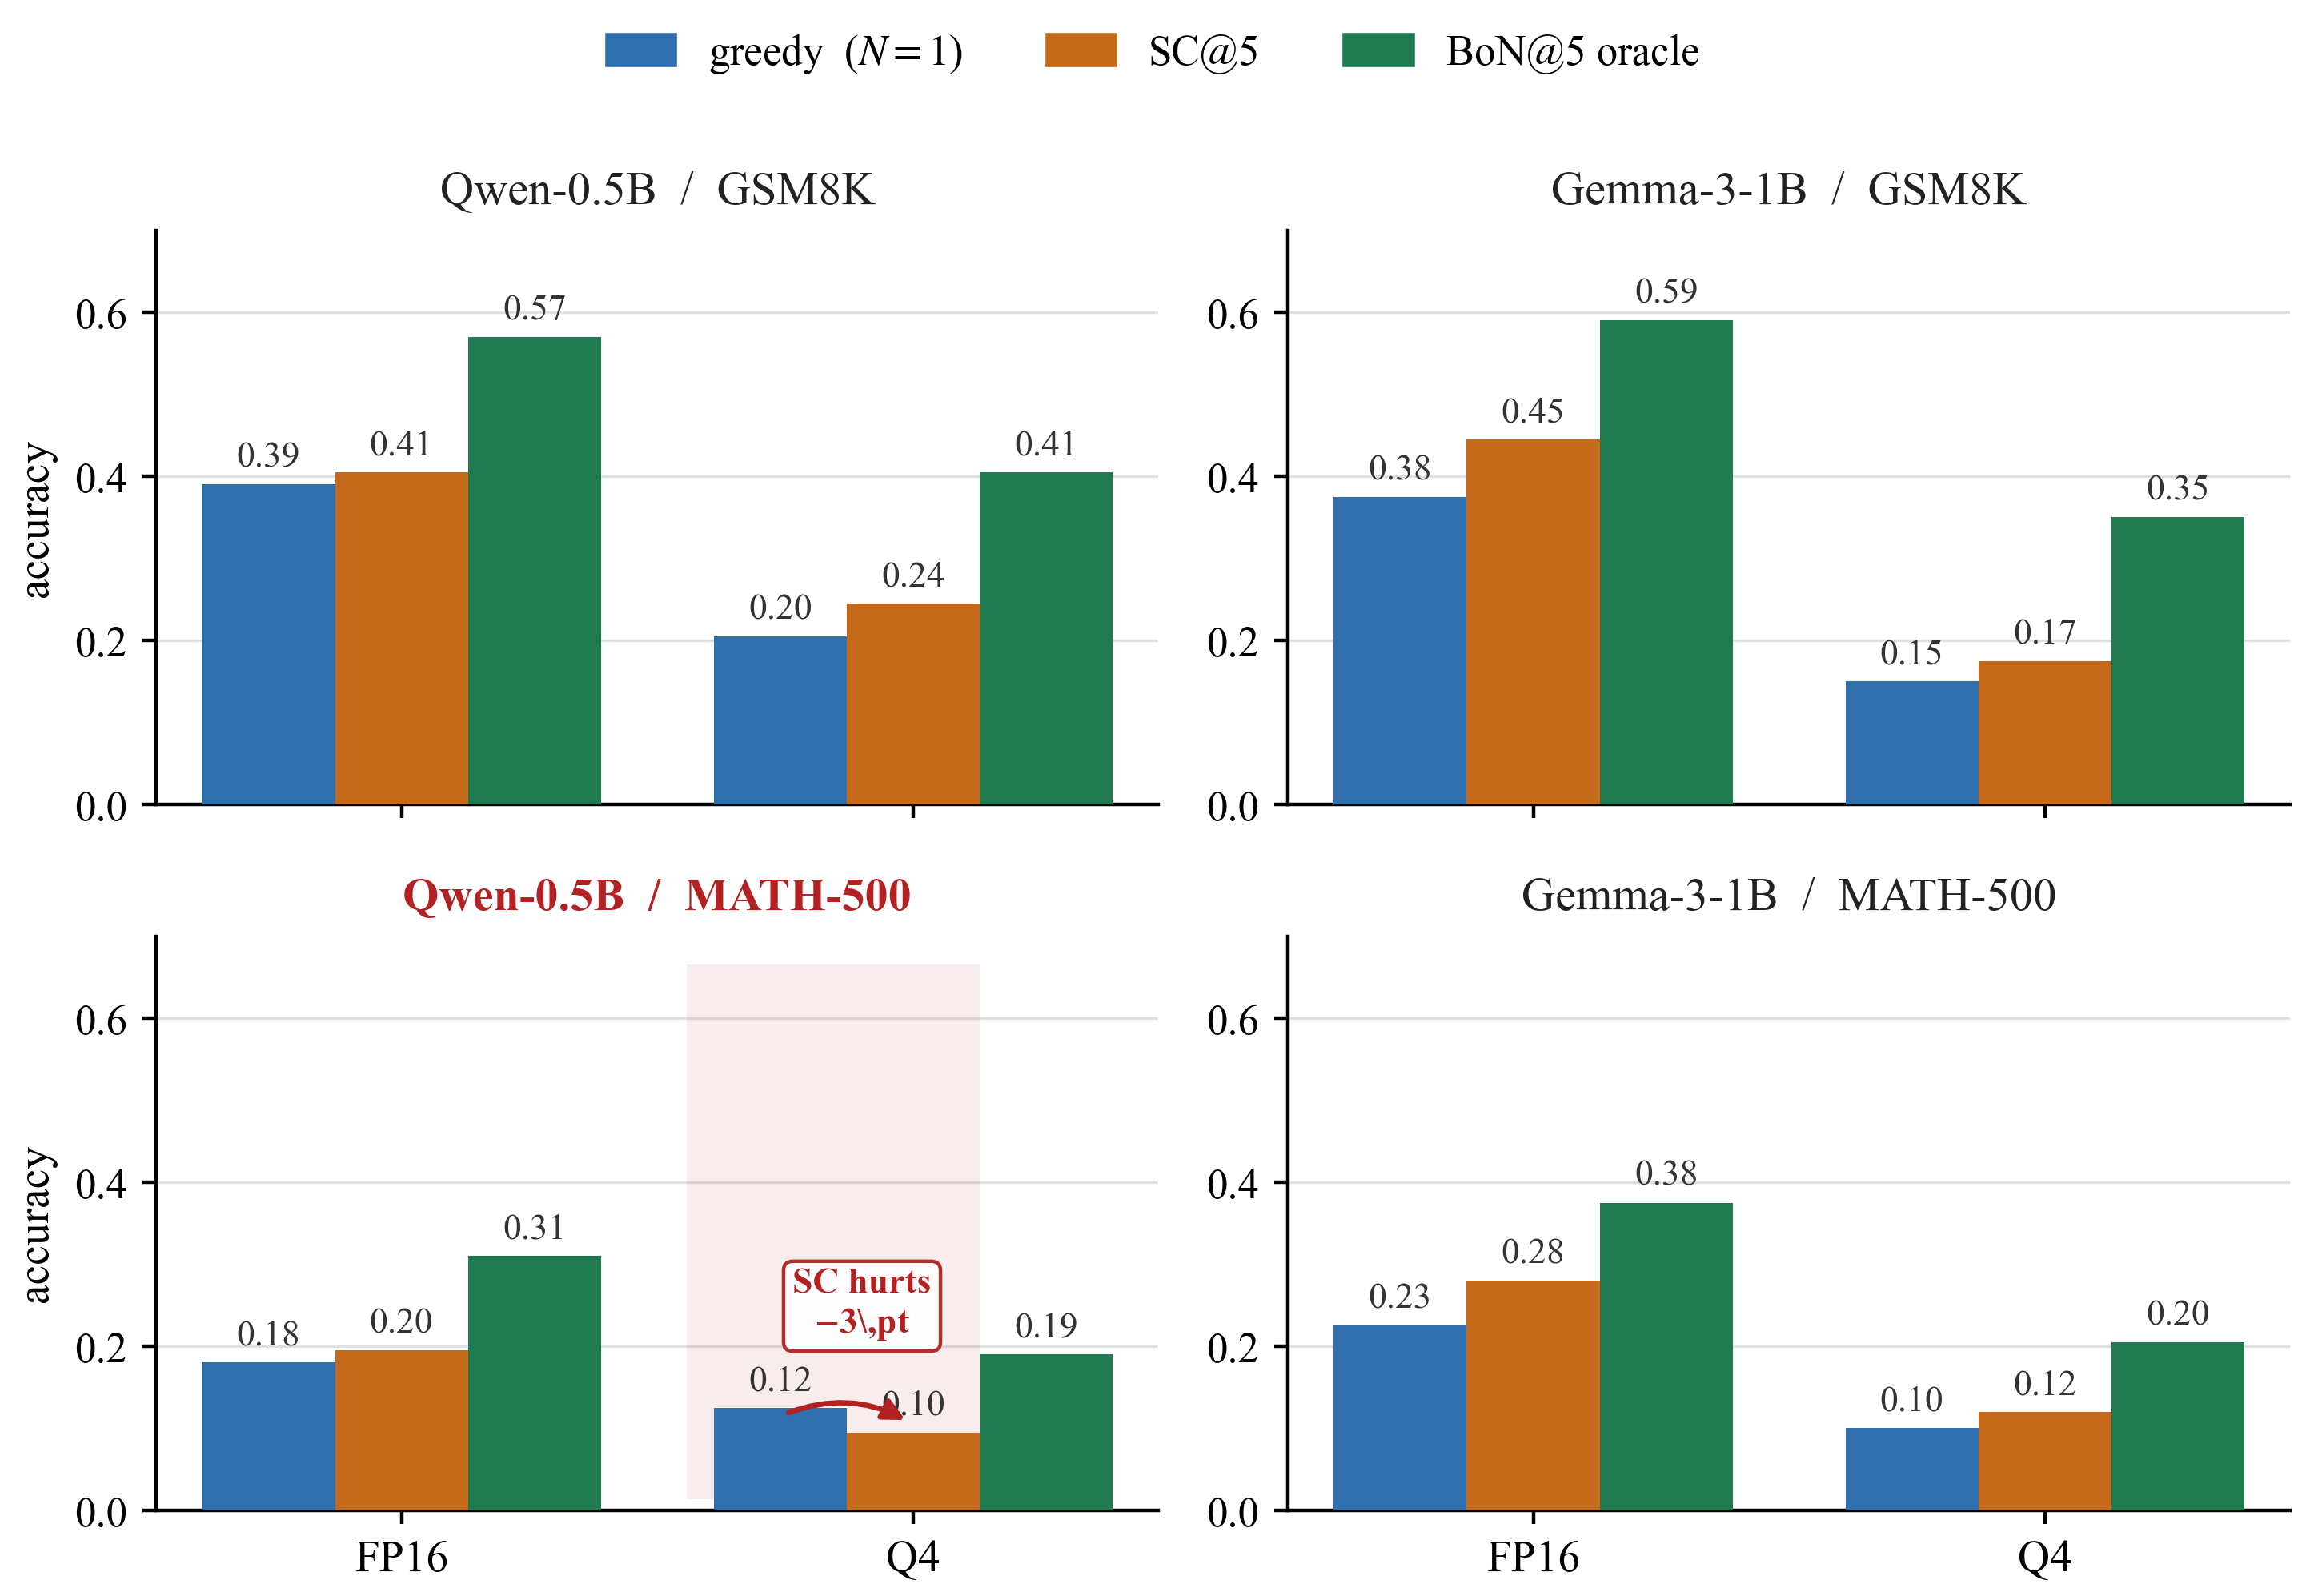
\includegraphics[width=\textwidth]{fig3_fp16_vs_q4.png}
\caption{Greedy, SC@5, and BoN@5 oracle accuracies per
(family,~dataset,~precision). 4-bit MLX quantisation drops greedy
accuracy by 5--22\,pt (paired bootstrap CIs non-overlapping 0); SC@5
gain (SC@5 $-$ greedy) is small (1.5--7\,pt) and \emph{negative} on
Qwen-Q4${\times}$MATH-500 ($-3\,\text{pt}$).}
\label{fig:quant}
\end{figure*}

\begin{table}[t]
\centering\small
\begin{tabular}{llccr}
\toprule
Cell & Dataset & $y$ & $h$ & sc\_gain \\
\midrule
Qwen-FP16  & GSM8K    & 12.0\% & 10.5\% & $+1.5$ \\
Qwen-Q4    & GSM8K    & 12.5\% &  8.5\% & $+4.0$ \\
Gemma-FP16 & GSM8K    & 11.0\% &  4.0\% & $+7.0$ \\
Gemma-Q4   & GSM8K    &  7.0\% &  4.5\% & $+2.5$ \\
Qwen-FP16  & MATH-500 &  6.0\% &  4.5\% & $+1.5$ \\
\textbf{Qwen-Q4} & \textbf{MATH-500} &  4.0\% &  7.0\% & $\mathbf{-3.0}$ \\
Gemma-FP16 & MATH-500 &  9.0\% &  3.5\% & $+5.5$ \\
Gemma-Q4   & MATH-500 &  5.0\% &  3.0\% & $+2.0$ \\
\bottomrule
\end{tabular}
\caption{Per-prompt decomposition of SC's verdicts. $y$=SC helps,
$h$=SC hurts. sc\_gain (pt) $=y-h$. On Qwen-Q4${\times}$MATH, $h>y$ so
SC actively hurts.}
\label{tab:yh}
\end{table}

Oracle retention $\in[109\%,174\%]$ on all 12 experiments. On
\textbf{Qwen-Q4${\times}$MATH-500}, oracle retention is
$174\%$: always-SC leaves 7\,pt of accessible accuracy on the
table. Figure~\ref{fig:quant} shows the raw accuracies: 4-bit
quantisation drops greedy by 5--22\,pt (all paired bootstrap CIs
non-overlapping zero, see App.~B), and SC@5 gain is marginal to
negative everywhere.

\subsection{When does SC hurt?}

Table~\ref{tab:yh} decomposes per-prompt verdicts. The $y$ rate (SC
helps) is 4--12\%; the $h$ rate (SC hurts) is 2--13\%. On
Qwen-Q4${\times}$MATH, $h$ exceeds $y$ by 3\,pt, inverting the sign of
sc\_gain. This is not model-specific pathology --- it is a property of
plurality voting under imperfect calibration when multiple distinct
candidate answers emerge per prompt.

\section{The TTC-Gate}
\label{sec:method}

\subsection{Problem statement}

A \textbf{TTC-gate} is a scalar score $s{:}~\text{prompt}\to[0,1]$
computed from the greedy pass. For threshold $\tau$:
\begin{itemize}
  \itemsep 0em
  \item $s(x) \ge \tau$: run SC@5 (cost $5{\times}$, accept SC).
  \item $s(x)   < \tau$: skip SC (cost $1{\times}$, accept greedy).
\end{itemize}

We study three gate instances.
\textsc{conf\_only}: $s(x){=}1-\text{greedy\_margin\_confidence}(x)$,
the mean top-1 minus top-2 softmax probability over greedy-generated
tokens. No learning; $\tau$ is the only parameter.
\textsc{logistic}: L2-regularised, class-balanced logistic regression on
12 features: 4 greedy aggregates (conf, top-5 entropy, full-vocab
entropy, token count) + 8 prompt-text features (length, digit count,
operator count, comma count, newline count, step-marker count).
\textsc{mlp}: a 32$\times$16 hidden-layer MLP on the same 12 features,
L2-regularised.

All gates are trained via 5-fold CV within each cell, producing
out-of-fold scores. We pick the operating threshold $\tau$ that
maximises skip-rate subject to $\text{acc\_retention}\ge 0.98$ on the
full out-of-fold data, then bootstrap $1\,000{\times}$ over prompts at
the fixed $\tau$ for CIs.

\subsection{Pooled results}

\begin{figure*}[t]
\centering
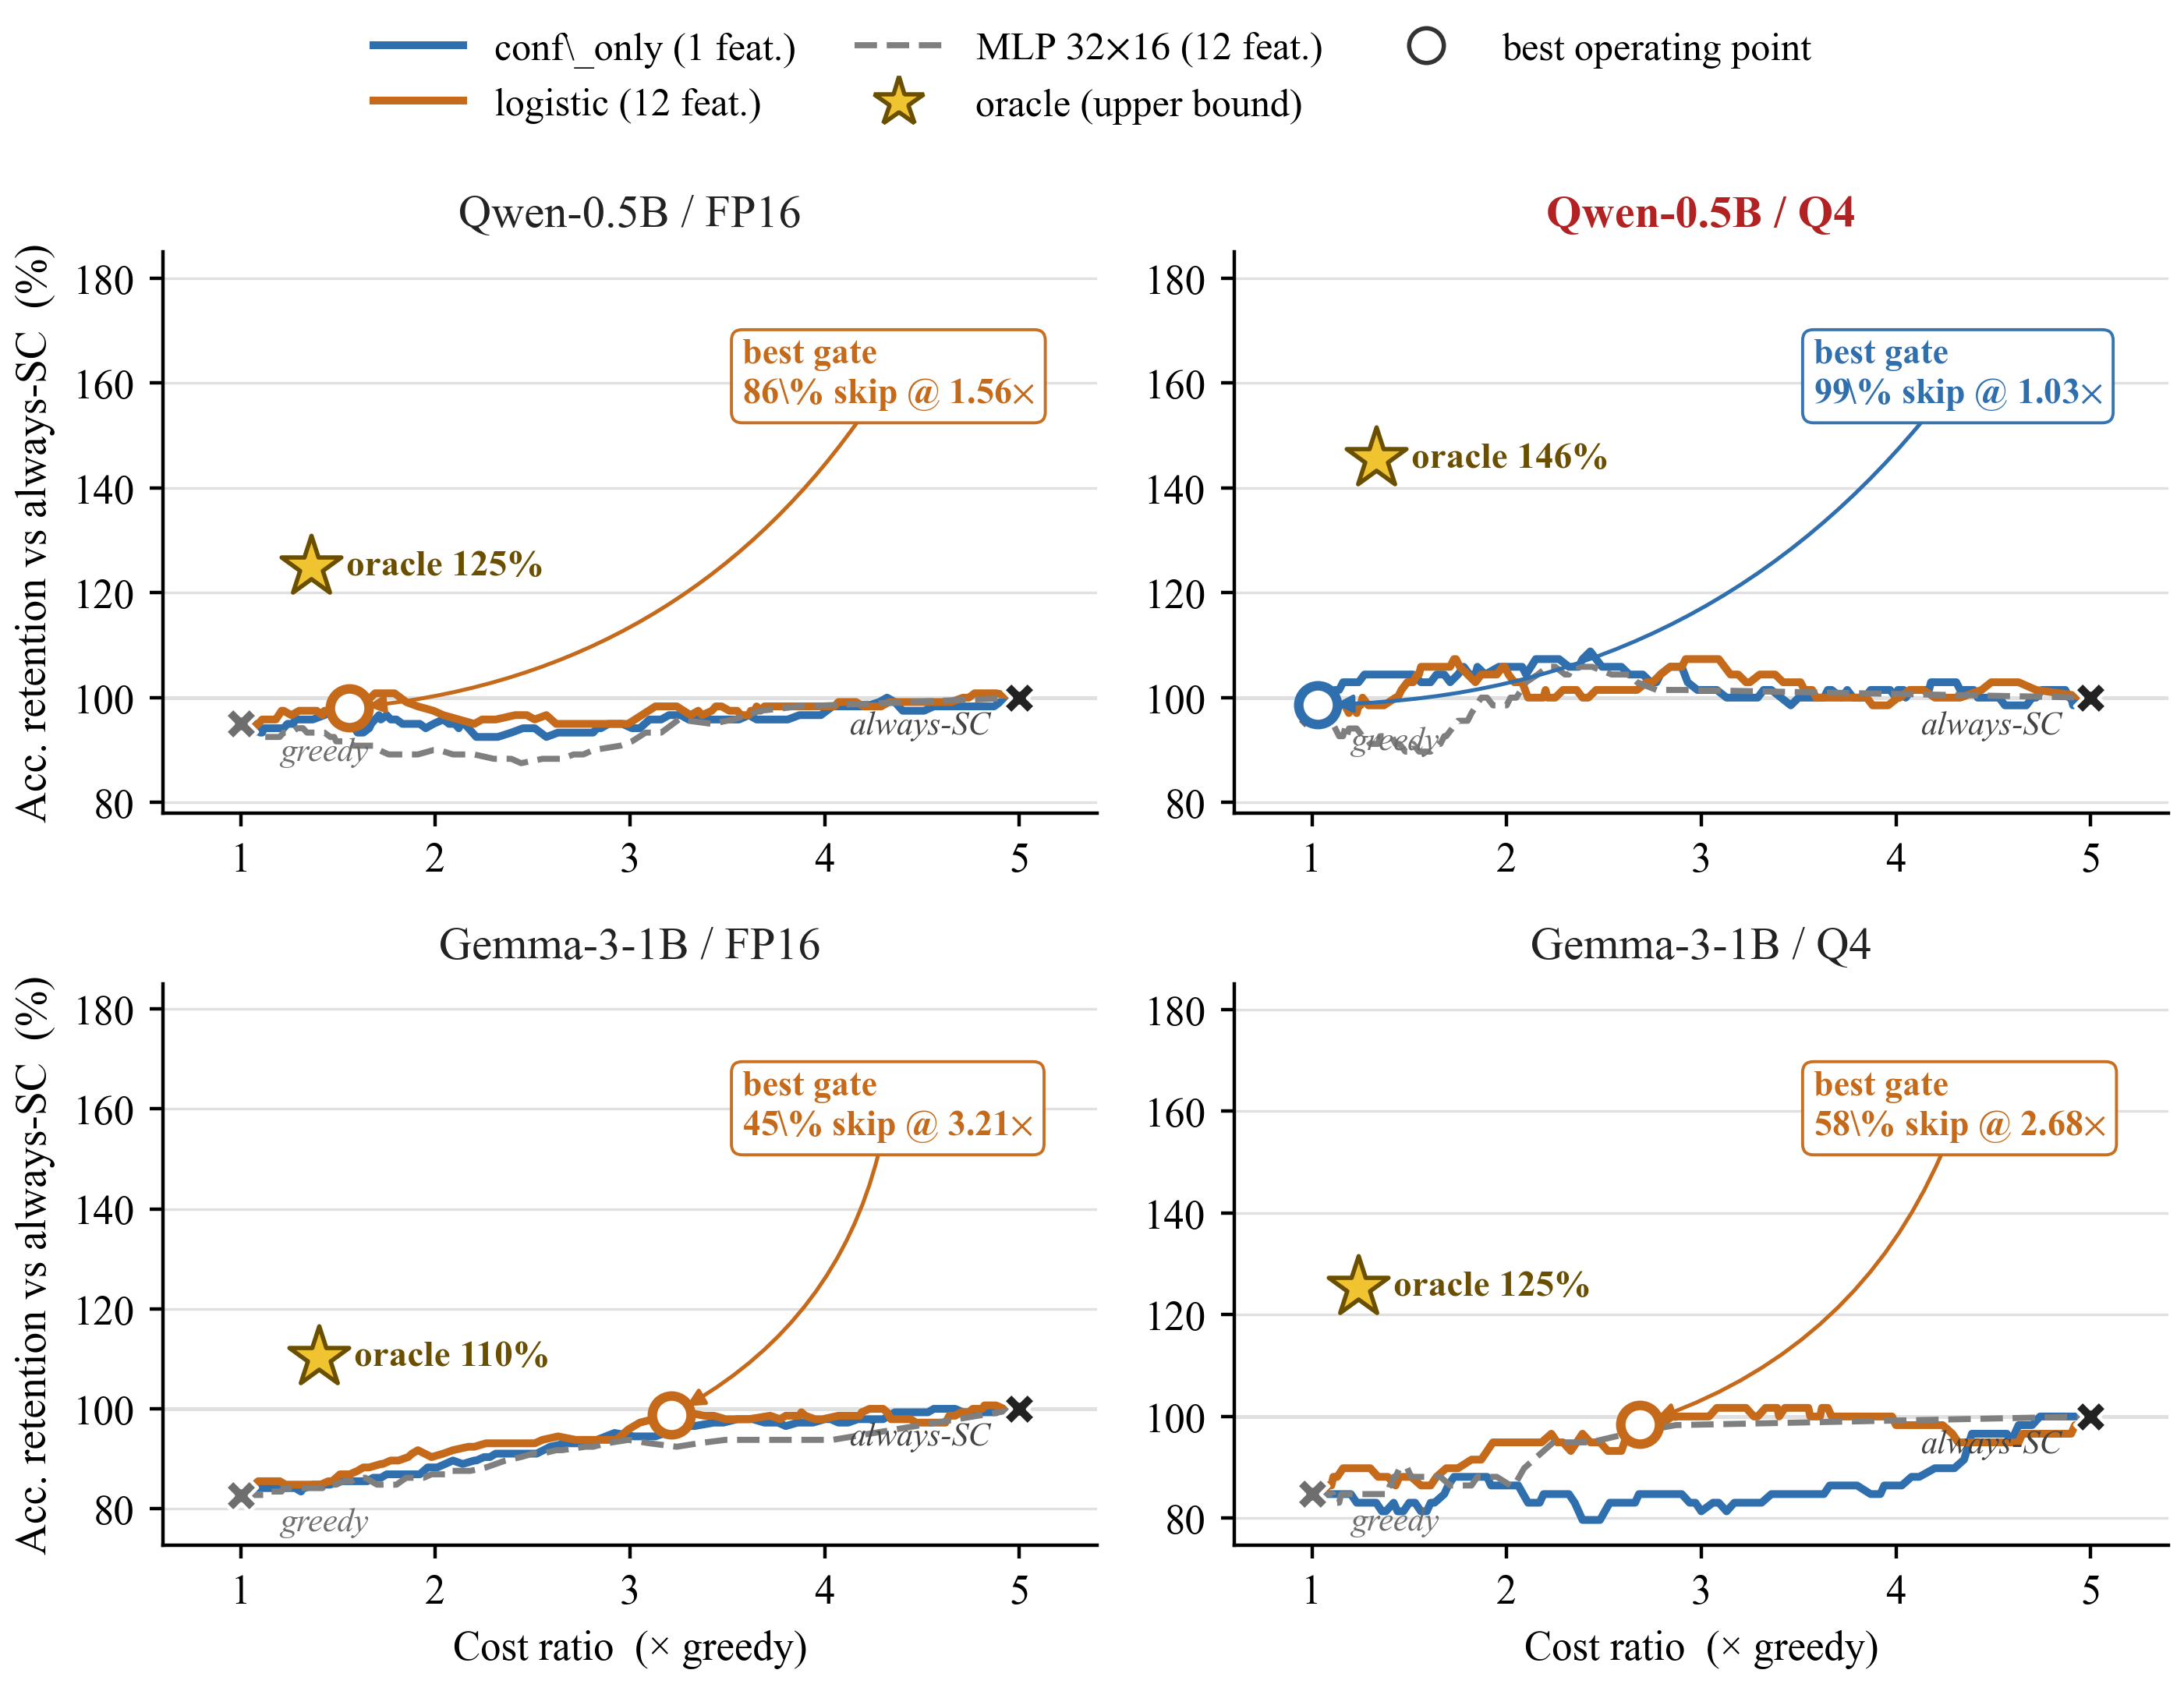
\includegraphics[width=0.85\textwidth]{fig2_pareto_pooled.png}
\caption{TTC-Gate Pareto curves on the four pooled cells
($n{=}400$ per cell). Each curve traces $\tau$ across the
(cost~ratio, acc~retention) plane. Gold star: oracle upper bound;
hollow circle: best operating point at retention~$\ge 98\%$.
Italic labels mark always-greedy (cost $1{\times}$) and always-SC
(cost $5{\times}$). \textsc{Logistic} (12 features) outperforms
\textsc{conf\_only} on 3/4 cells at pooled scale; MLP loses
universally.}
\label{fig:pareto}
\end{figure*}

\begin{table*}[t]
\centering\small
\begin{tabular}{lcccccc}
\toprule
Cell & Method & $\tau$ & skip \% [CI] & cost$\times$ [CI] & retention \% [CI] \\
\midrule
Qwen-FP16  & logistic  & 0.625 & 86.0 [82.5, 89.3] & 1.56 [1.43, 1.70] & 98.1 [82.5, 112.5] \\
Qwen-Q4    & conf\_only & 0.915 & 99.3 [98.5, 100.0] & 1.03 [1.00, 1.06] & 98.7 [76.5, 120.6] \\
Gemma-FP16 & logistic  & 0.46  & 44.7 [40.0, 49.5]  & 3.21 [3.02, 3.40] & 98.8 [86.2, 112.4] \\
Gemma-Q4   & logistic  & 0.515 & 57.9 [53.2, 62.7]  & 2.68 [2.49, 2.87] & 98.5 [77.9, 122.0] \\
\bottomrule
\end{tabular}
\caption{Pooled ($n{=}400$) TTC-gate operating points. $\tau$ chosen
for max skip-rate s.t.\ retention $\ge 98\%$. Best gate saves
\textbf{45--99\%} compute with $\ge 98\%$ retention. Bootstrap
($1\,000{\times}$) CIs in brackets; skip-rate CIs are tight
($\pm 3$--$4$\,pt), retention CIs are wider because the denominator
(SC@5 accuracy) is small on these models.}
\label{tab:gate-pooled}
\end{table*}

Figure~\ref{fig:pareto} shows the Pareto curves for the four pooled
cells. Table~\ref{tab:gate-pooled} reports the best operating point
per cell with 95\% CIs. Across all four cells the best gate saves
\textbf{45--99\%} of the always-SC compute while retaining
$\ge 98\%$ of its accuracy. On Qwen-Q4 the gate effectively becomes
``always greedy with a sliver of SC calls'' (99.3\% skip): it has
learned that SC is net-negative for this cell and disables itself.

\subsection{Feature ablation}
\label{sec:ablation}

We compare \textsc{conf\_only} (1 feature), \textsc{logistic} (12
features), \textsc{mlp} (12 features, 32$\times$16 hidden) at both the
$n{=}200$ per-task and $n{=}400$ pooled scales.

\begin{enumerate}
  \item \textbf{At $n{=}200$ per cell}, \textsc{conf\_only} is frequently
        the best gate; \textsc{logistic} is competitive; \textsc{mlp}
        often collapses to $\tau{=}0$ because the class-balanced
        training signal is thin at $n{=}160$ training prompts with
        $10\text{--}20$ positive labels.
  \item \textbf{At $n{=}400$ pooled}, \textsc{logistic} overtakes
        \textsc{conf\_only} on 3/4 cells: with more training data the
        linear combination of the 12 features beats the single
        strongest one.
  \item \textbf{\textsc{mlp} never wins at any scale} in our
        experiments. The decision surface is essentially linear in
        scaled features; extra capacity over-fits.
\end{enumerate}

\begin{table}[t]
\centering\small
\begin{tabular}{lc}
\toprule
Feature & coefficient \\
\midrule
greedy\_mean\_ent  & $+0.71$ \\
greedy\_top5\_ent  & $+0.58$ \\
greedy\_conf       & $-0.52$ \\
text\_n\_ops       & $+0.31$ \\
text\_n\_digits    & $+0.19$ \\
\bottomrule
\end{tabular}
\caption{Top-5 standardised-feature coefficients from the pooled
Qwen-FP16 \textsc{logistic} gate. Positive~$\to$~higher score~$\to$~more
likely to run SC. High entropy and low margin (high uncertainty)
correctly flag SC-worthiness.}
\label{tab:coef}
\end{table}

Table~\ref{tab:coef} gives the top-5 standardised-feature coefficients
of the pooled Qwen-FP16 \textsc{logistic} model. The dominant signals
are greedy token-level entropy (positive, more entropy $\to$ run SC)
and greedy margin confidence (negative, more confident $\to$ skip).
Operator and digit counts provide residual signal.

\begin{figure*}[t]
\centering
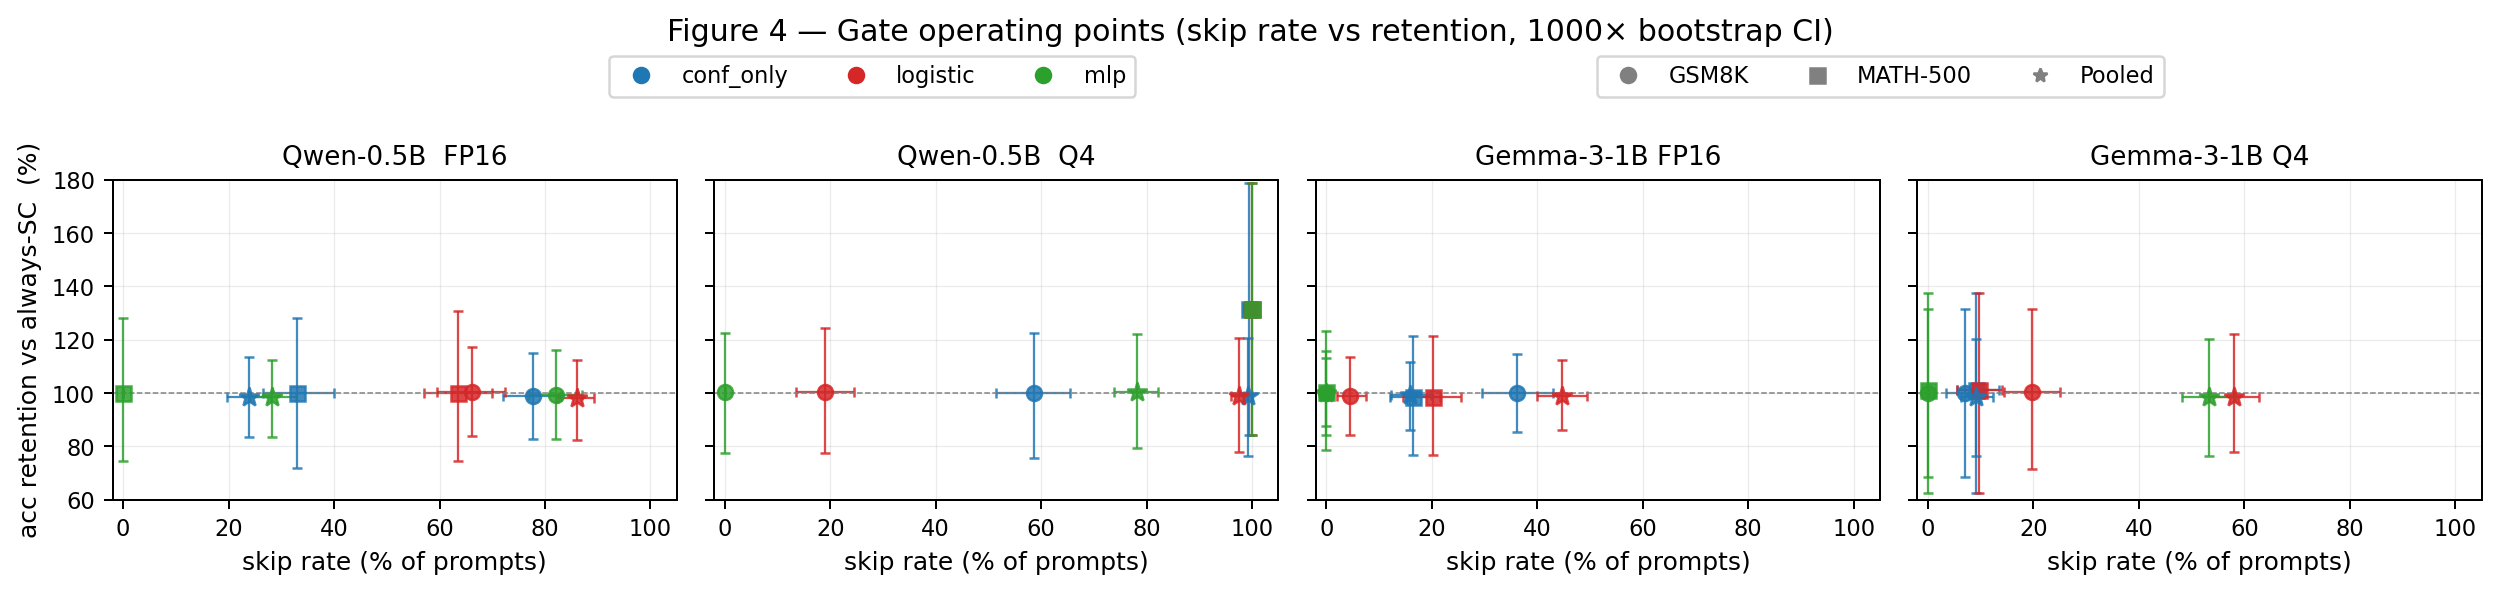
\includegraphics[width=\textwidth]{fig4_operating_points.png}
\caption{Operating points (skip rate vs.\ retention) per
(cell, method, dataset) with $1\,000{\times}$ bootstrap CI bars.
Pooled points (stars) have the tightest CIs. Method ranking is
stable: \textsc{logistic} $\gtrsim$ \textsc{conf\_only} $\gg$
\textsc{mlp}.}
\label{fig:operating}
\end{figure*}

Figure~\ref{fig:operating} plots the (skip\_rate, retention) bootstrap
point per cell, method, and dataset. Pooled stars give the tightest CIs; per-task markers are noisier. Method ranking is stable.

\section{Discussion}

\paragraph{Why do small models fail always-SC?}
The harm rate $h$ requires a wrong answer to win a plurality vote over
the correct one. This happens when (i) the model's distribution over
candidate answers is diffuse, and (ii) the wrong-majority mode is
entropically cheap under the sampler. On small models both conditions
hold on hard prompts. SC's strength on large models is that both rates
are low and $y - h$ is consistently positive; on small models the
rates are small and comparable.

\paragraph{Why is Gemma's gate weaker than Qwen's?}
Across 2 datasets and both precisions, Qwen gates save 33--99\% of
compute while Gemma gates save 17--58\%. Two hypotheses: (a) Gemma-3's
RLHF may have compressed its greedy confidence into a narrower range,
reducing feature informativeness; (b) Gemma-3's sliding-window
attention \citep{Gemma3Report} may interact with greedy token margins
differently. We did not do a controlled analysis; a natural follow-up.

\paragraph{Why do deeper MLPs lose?}
Per-cell $n{=}160$ (training fold) with 12 features and 3\% positive
base-rate is firmly in linear-model territory. Extra nonlinearity is
over-parameterisation.

\section*{Limitations}

\begin{enumerate}
\itemsep 0em
\item \textbf{One random seed.} Pooled $n{=}400$ already tightens
      skip-rate CIs to $\pm 3$\,pt, but acc-retention CIs remain wide
      because SC-accuracy is small (ratio variance dominates). Three
      seeds would tighten retention further.
\item \textbf{Two model families, two math benchmarks.} Generalisation
      to coding, commonsense, retrieval-heavy tasks, or 3B+ models is
      not tested.
\item \textbf{SC@5 only.} At $N{=}16$ / $N{=}32$ the gate may need
      retuning; the harm rate $h$ likely falls as $N$ grows.
\item \textbf{Fixed threshold.} Adaptive $\tau$ by prompt-difficulty
      bucket is an obvious extension.
\item \textbf{Not verifier-aware.} If a cheap verifier is available
      post-SC, the right analysis is a three-way gate
      (greedy~/~SC~/~SC$+$verifier); we leave this to future work.
\end{enumerate}

\section{Conclusion}

On small ($<$2B) reasoning models, the default ``always SC'' recipe is
dominated by a per-prompt oracle gate in every one of our 12
experiments. The mechanism is a non-negligible rate of SC flipping
correct answers to wrong --- a pathology that plurality voting cannot
detect. We show that a 12-feature logistic gate, trained on a few
hundred calibration prompts, realises most of the oracle's savings
(45--99\% in the pooled $n{=}400$ analysis) at $\ge 98\%$ accuracy
retention. The gate is model-local, verifier-free, runs on-device,
and is deploy-ready. Before reporting ``SC@$N$ improves accuracy'' on
small models, check the harm rate.

% Bibliography
\bibliography{custom}

\appendix

\section{Reproducibility}
\label{sec:appendix}

All experiments run on a single MacBook Pro M4 Pro (24\,GB unified
memory, Apple M4 GPU, MLX 0.31 + \texttt{mlx-lm} 0.31 + PyTorch 2.11
with MPS, Python 3.13). Wall-clock budget:

\begin{itemize}
  \itemsep 0em
  \item Block A generation, GSM8K (4 cells $\times$ 200 prompts
        $\times$ 6 gens): 3\,h 00\,min.
  \item Block A generation, MATH-500: 4\,h 30\,min.
  \item Consolidation scripts (bootstrap $1\,000{\times}$, featurise,
        fit, figure): $<$3\,min.
\end{itemize}

Total GPU-hours: $\approx 7.5$. No CUDA, no cloud, no paid API.

\section{Per-cell paired FP16-vs-Q4 bootstrap}
\label{sec:appendix-b}

Full $1\,000{\times}$ paired bootstrap of FP16-minus-Q4 differences,
$n{=}200$ per cell.

\begin{table}[h]
\centering\small
\begin{tabular}{lllcc}
\toprule
Dataset & Model & Metric & $\Delta$ & 95\% CI \\
\midrule
GSM8K    & Qwen  & greedy & $+0.186$ & $[+0.110, +0.265]$ \\
GSM8K    & Qwen  & SC@5   & $+0.160$ & $[+0.095, +0.230]$ \\
GSM8K    & Gemma & greedy & $+0.224$ & $[+0.160, +0.290]$ \\
GSM8K    & Gemma & SC@5   & $+0.270$ & $[+0.205, +0.340]$ \\
MATH-500 & Qwen  & greedy & $+0.055$ & $[+0.005, +0.105]$ \\
MATH-500 & Qwen  & SC@5   & $+0.099$ & $[+0.055, +0.145]$ \\
MATH-500 & Gemma & greedy & $+0.124$ & $[+0.075, +0.175]$ \\
MATH-500 & Gemma & SC@5   & $+0.159$ & $[+0.105, +0.220]$ \\
\bottomrule
\end{tabular}
\caption{Paired FP16$-$Q4 contrasts. All 8 have non-overlapping-zero
95\% CIs.}
\end{table}

\end{document}
